%----------------------------------------------------------------------------------------
%	IMPLEMENTAZIONE
%----------------------------------------------------------------------------------------

\section{Implementazione}
\label{sec:implementazione}

In questo capitolo vengono dettagliate le scelte implementative alla base del software di simulazione. Pur non trattando singolarmente ciascuna di esse, si cercherà di mettere in evidenza i punti più significativi, sia nell'ottica della concorrenza che nell'ottica della distribuzione.

\subsection{Concorrenza}
\label{sec:implemetazione_concorrenza}

Questa sezione consta di alcuni aspetti implementativi legati alla concorrenza del sistema. In particolare, saranno dettagliati i seguenti aspetti:

\begin{itemize}
	\item avvio del sistema;
	\item riaccodamento dei giocatori;
	\item terminazione del sistema.
\end{itemize}

Verrà infine illustrato un diagramma di sequenza che focalizza alcuni degli aspetti sopra elencati.\\

\subsubsection{Avvio del sistema}
\label{sec:implementazione_concorrenza_avvio_sistema}

L'avvio del sistema prevede, per quanto riguarda la parte \emph{Core}, l'inizializzazione di diverse componenti, prime fra tutti i giocatori: i 22 task di tipo Player vengono avviati simultaneamente nel \verb+main+ del software (il begin corrisponde quindi ad un co-begin) e, dal momento che sono le uniche entità attive del sistema, la loro terminazione determinerà la terminazione di tutto il software.\\

Dal momento che l'inizio di una partita prevede prima una configurazione delle squadre e dei relativi giocatori, i 22 task si accodano inizialmente su una risorsa protetta chiamata \emph{GameEntity} attraverso il canale \verb+Rest+, la cui guardia si apre solamente quando arriva il segnale di inizio di una nuova partita o di inizio del secondo tempo. Alla sua apertura, i task recuperano il proprio identificativo attraverso il canale \verb+GetId+ del controllore, che corrisponde ad uno dei giocatori in campo. A questo punto, i giocatori fanno il loro ingresso in campo e, una volta raggiunta la loro posizione di riferimento, si accodano nuovamente su \emph{GameEntity}: la guardia del canale \verb+Start1T+ si apre solamente quando l'arbitro ha decretato che tutti i giocatori sono in posizione e che la partita è pronta per cominciare. I giocatori procedono quindi il loro ciclo di lettura dello stato, decisione della prossima mossa e successiva scrittura sullo stato.\\

\subsubsection{Riaccodamento}
\label{sec:implementazione_concorrenza_riaccodamento}

Nel Capitolo~\ref{sec:analisi_architetturale} si è parlato di come possa accadere che una mossa non sia soddisfacibile al momento della richiesta. La mossa, a seconda della sua tipologia e dell'utilità assegnatavi, può essere rivalutata con una mossa che si avvicini il più possibile alla richiesta originale del giocatore. D'altro canto, ci sono circostanze in cui la mossa è necessaria e una sua rivalutazione causerebbe un comportamento di gioco lontano dalla realtà.\\

Il meccanismo che realizza il riaccodamento per una mossa momentaneamente non attuabile utilizza una risorsa protetta chiamata \emph{Guard}, che mette a disposizione due canali: \verb+Wait+ e \verb+Update+. Un giocatore la cui mossa non può essere eseguita viene riaccodata su tale risorsa attraverso il canale \verb+Wait+, in attesa che venga eseguita un'azione di movimento (l'unico tipo di azione rivalutabile) sulla zona di campo corrispondente. Dualmente, ogni volta che un giocatore effettua un'azione di movimento, aggiorna \emph{Guard} notificando il movimento in quella particolare zona di campo. Si ha così che, nel caso di azioni di movimento in attesa, esse non vengono ``risvegliate'' ad ogni altro movimento di un giocatore, ma sono localizzate in una specifica zona di campo.\\

\subsubsection{Terminazione del sistema}
\label{sec:implementazione_concorrenza_terminazione_sistema}

La terminazione del sistema viene richiesta dall'utente, attraverso i comandi messi a disposizione nell'interfaccia grafica di \emph{Field}. Una volta ricevuta da \emph{Core}, il controllore fa in modo di inoltrarla anche alle due istanze di \emph{Manager}, che termineranno di conseguenza la loro esecuzione. Inoltre, il controllore aggiorna lo stato in maniera da notificare ai giocatori la richiesta di terminazione. Infine, il controllore richiede la terminazione del software attraverso la procedura \verb+Exit_Program+.\\

\subsubsection{Diagramma di sequenza}
\label{sec:implementazione_concorrenza_diagramma_sequenza}

\begin{figure}[htp!]
	\centering
	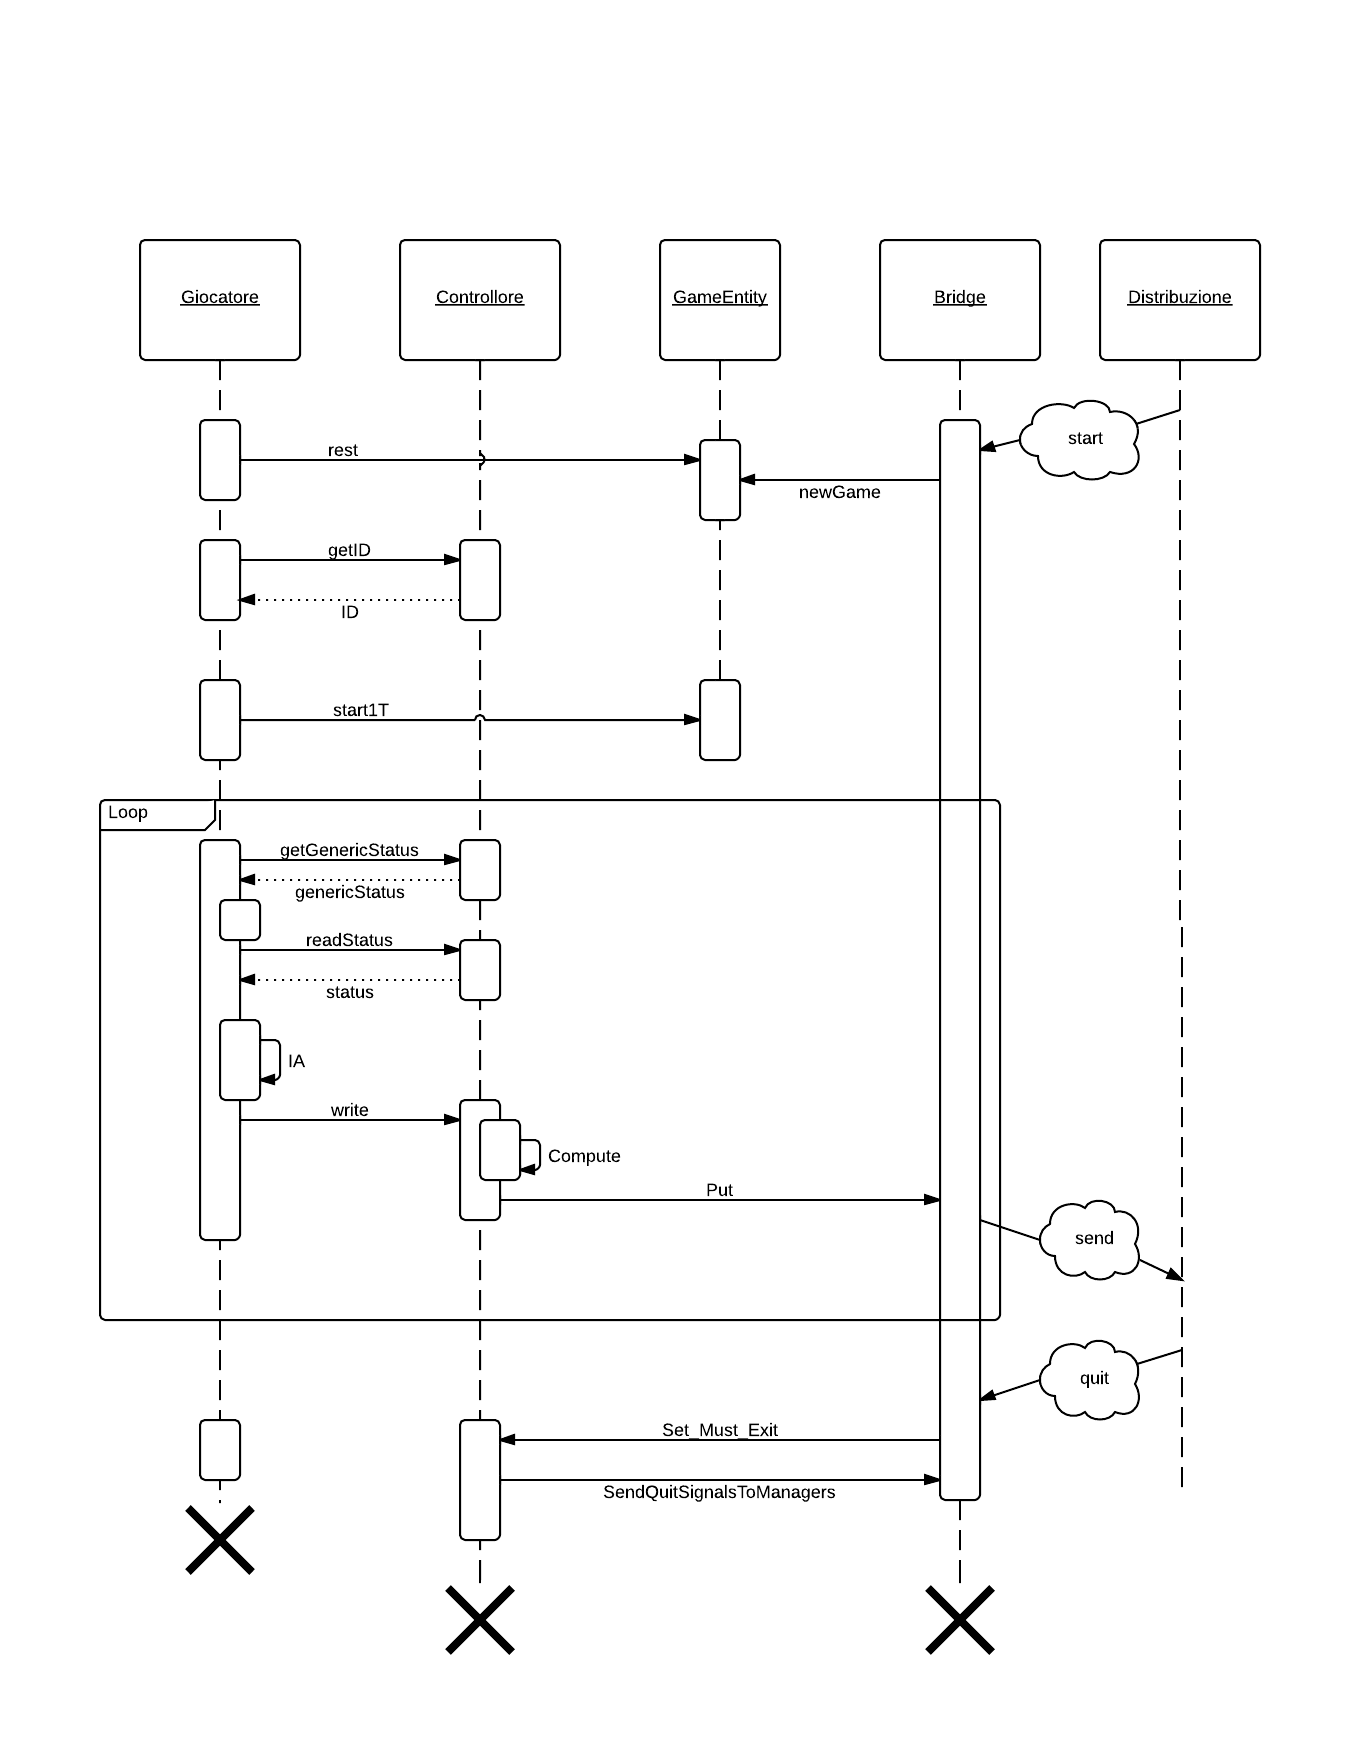
\includegraphics[scale=.35]{images/system_sequence_diagram}
	\caption{Diagramma di sequenza che comprende avvio del sistema, mossa di un giocatore e terminazione del sistema.}
	\label{fig:sequence_diagram}
\end{figure}

Il diagramma di sequenza mostrato in Figura~\ref{fig:sequence_diagram} schematizza il flusso base della simulazione. In esso viene rappresentato l'avvio del sistema, che comprende la creazione dei task per i giocatori e l'assegnamento dei loro identificativi. Con il loop centrale si identifica il turno di un giocatore.

\subsection{Distribuzione}
\label{sec:implementazione_distribuzione}

La comunicazione tra la componente \emph{Core} e le componenti \emph{Field} e \emph{Manager} è stata realizzando aggiungendo un modulo a \emph{Core} che agisce come web server. Per rendere possibile questa interazione si è ricorsi all'utilizzo di AWS (Ada Web Server). All'avvio del sistema, viene inizializzato un web server su \emph{localhost:28000}, a cui \emph{Field} e \emph{Manager} si connettono e con il quale successivamente scambiano informazioni.\\

Come già illustrato in Sezione~\ref{sec:analisi_client_server}, la comunicazione tra le componenti distribuite \emph{Field} e \emph{Manager} e la componente centrale \emph{Core} è stata implementata con un modello di comunicazione tipico di un’architettura client-server. Si ha quindi che ciascuna istanza di \emph{Manager}, una volta avviata, invia una richiesta HTTP di tipo GET a \emph{Core}, richiedendo le statistiche dei giocatori della squadra. La componente \emph{Field} effettua invece chiamate HTTP di tipo GET verso \emph{Core} al fine di richiedere azioni quali l'avvio di una nuova partita, l'avvio del secondo tempo della partita corrente, la messa in pausa della partita corrente, ed infine la terminazione forzata della partita.\\

Dal momento che \textit{Manager} e \textit{Field} sono state realizzate in Java, per facilitare tale tipo di comunicazione è stata utilizzata la libreria open source Apache HttpComponents, che fornisce una completa implementazione del protocollo HTTP in Java e consente di avere accesso a funzionalità avanzate e maggiore flessibilità rispetto al package standard \emph{java.net} di Java.\\

In generale, le richieste provenienti da \emph{Field} e \emph{Manager} sono inizialmente ricevute dal modulo \emph{Soccer.Server.Callbacks} che si occupa di verificare di quale tipo di richiesta si tratta (i metodi a disposizione delle componenti distribuite sono consultabili in sezione ~\ref{sec:analisi_distribuzione_bridge_input}), per poi inoltrarla correttamente verso la componente \emph{Core} tramite il modulo bridge input. Nel caso in cui il client richiedente attenda una risposta da \emph{Core} (e.g. il client ha chiesto le statistiche dei giocatori), il modulo \emph{Soccer.Server.Callbacks} si occuper\`{a} di fornirla al client.\\

La comunicazione di \emph{Core} con le componenti distribuite \emph{Field} e \emph{Manager} è invece vista come un modello di comunicazione di tipo publisher-subscriber. \emph{Core} mette infatti a disposizione i seguenti canali di comunicazione ai quali le componenti interessate si iscrivono per ricevere informazioni:

\begin{itemize}
	\item \emph{/managerVisitors/registerForStatistics} \`{e} il socket su cui una delle istanze di \emph{Manager} rimane in ascolto, in particolare l'istanza che rappresenta la squadra che gioca ``fuori casa'';
	\item \emph{/managerHome/registerForStatistics} \`{e} il socket su cui una delle istanze di \emph{Manager} rimane in ascolto, in particolare l'istanza che rappresenta la squadra che gioca ``in casa'';
	\item \emph{/field/registerForEvents} \`{e} il socket a cui si connette \emph{Field}.
\end{itemize}

Per realizzare questo tipo di comunicazione si è deciso di utilizzare la tecnologia dei WebSocket. Questo particolare tipo di socket mantiene attivo un canale di comunicazione tra due componenti, ad esempio \emph{Core} e \emph{Field}, permettendo cosî la fruizione di contenuti di \emph{Core} da parte di \emph{Field}. Il principale vantaggio nell'utilizzo dei WebSocket consiste nel fatto che l'invio di nuovi contenuti disponibili da parte dell'entità produttore verso le entità consumatore avviene senza alcuna richiesta o sollecitazione da parte di questi ultimi: non appena è disponibile un nuovo contenuto, il produttore lo invia autonomamente ai consumatori, i quali sono in ascolto sui corrispondenti WebSocket aperti. Le istanze di \emph{Manager} riceveranno informazioni riguardanti le statistiche dei giocatori e la formazione della squadra, mentre \emph{Field} riceve tutti gli eventi correlati con la partita in corso.\\

In fase decisionale si è osservato che l'accoppiamento tra la componente \emph{Core} e il server per la comunicazione con le altre componenti potesse non essere desiderabile. Ad ogni modo, si è deciso di procedere ugualmente con questa decisione, sacrificando una parte di disaccoppiamento del sistema in favore dell'uso di una tecnologia relativamente nuova ed interessante come quella dei WebSocket, che è risultata essere estremamente affidabile e di facile utilizzo. Si noti che, al momento dell'integrazione, il supporto di Ada Web Server ai WebSocket era ancora molto sperimentale e non ufficializzato: fortunatamente, l'implementazione esistente vantava già un ottimo livello di stabilità.\\

Ada Web Server mette a disposizione una serie di API per facilitare l'uso dei WebSocket. Per aprire un nuovo socket è sufficiente utilizzare la funzione \emph{Register}, passando come parametro l'indirizzo su cui renderlo disponibile. Per inviare informazioni viene messa a disposizione la funzione \emph{Send}, specificando il WebSocket sul quale spedire i dati assieme alla tipologia di dato che si sta trasmettendo.\\

Come spiegato in sezione ~\ref{sec:analisi_distribuzione_bridge_output}, non vi è un continuo flusso di informazioni verso le componenti distribuite, ma viene utilizzato un buffer all'interno di bridge output, il cui scopo consiste nel bilanciare l'invio di dati: se da un lato un throughtput troppo basso comprometterebbe la rappresentazione grafica della partita, dall'altro un invio troppo frequente di aggiornamenti potrebbe causare una congestione di rete.

\subsubsection{Codifica delle Informazioni}

Tutti i messaggi scambiati secondo i modelli appena descritti sono codificati utilizzando il formato JSON, un formato di testo completamente indipendente dal linguaggio di programmazione, ma utilizza convenzioni conosciute dai programmatori di linguaggi della famiglia del C (come C/C++/C\#, Java/JavaScript e molti altri). Questa caratteristica fa di JSON un linguaggio ideale per lo scambio di dati.\\

La componente \emph{Core} processa i dati ricevuti in formato JSON utilizzando \emph{GNATColl}, o GNAT Component Collection, una libreria che mette a disposizione degli ADA package general purpose aggiuntivi. Tra di essi vi è il package \emph{GNATColl.JSON}, il quale permette sia la creazione di oggetti JSON che il parsing di tale tipo di dati ricevuti da \emph{Core}.\\

Per gestire le informazioni in formato JSON, le componenti distribuite, \emph{Manager} e \emph{Field}, utilizzano \emph{Gson}, una libreria open source  inizialmente sviluppata da Google. Questa libreria è stata scelta per la semplicità d'uso e la versatilità delle API messe a disposizione. La conversione di un oggetto Java nella sua rappresentazione in JSON è effettuata utilizzando il methodo \emph{toJson()} messo a disposizione dalla libreria. Similmente, la conversiona di una semplice stringa JSON nel corrispondente oggetto Java è resa possibile dal il metodo \emph{fromJson()}.

\subsubsection{Interfacce Grafiche}
Le GUI delle componenti \emph{Field} e \emph{Manager} sono state realizzate utilizzando il linguaggio Java. Questa scelta \`{e} stata guidata dal fatto che tale linguaggio garantisce un certo livello di portabilit\`{a} del sistema. In particolare, la grafica ed il layout sono stati implementati utilizzando il framework Swing.
